\documentclass{standalone}
\usepackage{tikz}
\usepackage{pgfplots}
\usetikzlibrary{spy}
\usetikzlibrary{backgrounds}
\usetikzlibrary{decorations}


\begin{document}
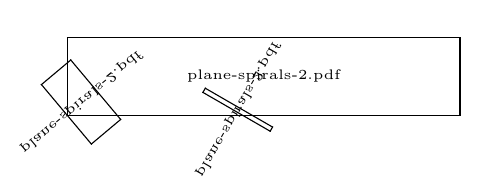
\begin{tikzpicture}
  \pgfdeclareimage[width=5cm]{swirl}{plane-spirals-2.pdf}
  \node () at (0,0) {\pgfuseimage{swirl}};
  \pgfdeclareimage[width=.5cm]{swirl2}{plane-spirals-2.pdf}
  \node[xscale=-1, rotate=140] () at (-2.32,-.327) {\pgfuseimage{swirl2}};


  \pgfdeclareimage[width=.075cm]{swirl3}{plane-spirals-2.pdf}
  \node[xscale=-1, rotate=120] () at (-.33,-.425) {\pgfuseimage{swirl3}};

  % \pgfdeclareimage[width=.1cm]{swirl2}{plane-spirals-2.pdf}
  % \node[rotate=-90] () at (-1,0) {\pgfuseimage{swirl2}};
  % \draw (-1.9, -.2) circle (.125);
  % \draw (-.2, -.2) circle (.0125);
  % \draw[latex-latex, ultra thin] (-3, -.425) -- (3, -.425);
\end{tikzpicture}
\end{document}
